\documentclass[]{article}
\usepackage{lmodern}
\usepackage{amssymb,amsmath}
\usepackage{ifxetex,ifluatex}
\usepackage{fixltx2e} % provides \textsubscript
\ifnum 0\ifxetex 1\fi\ifluatex 1\fi=0 % if pdftex
  \usepackage[T1]{fontenc}
  \usepackage[utf8]{inputenc}
\else % if luatex or xelatex
  \ifxetex
    \usepackage{mathspec}
    \usepackage{xltxtra,xunicode}
  \else
    \usepackage{fontspec}
  \fi
  \defaultfontfeatures{Mapping=tex-text,Scale=MatchLowercase}
  \newcommand{\euro}{€}
\fi
% use upquote if available, for straight quotes in verbatim environments
\IfFileExists{upquote.sty}{\usepackage{upquote}}{}
% use microtype if available
\IfFileExists{microtype.sty}{%
\usepackage{microtype}
\UseMicrotypeSet[protrusion]{basicmath} % disable protrusion for tt fonts
}{}
\usepackage[margin=1in]{geometry}
\usepackage{graphicx}
\makeatletter
\def\maxwidth{\ifdim\Gin@nat@width>\linewidth\linewidth\else\Gin@nat@width\fi}
\def\maxheight{\ifdim\Gin@nat@height>\textheight\textheight\else\Gin@nat@height\fi}
\makeatother
% Scale images if necessary, so that they will not overflow the page
% margins by default, and it is still possible to overwrite the defaults
% using explicit options in \includegraphics[width, height, ...]{}
\setkeys{Gin}{width=\maxwidth,height=\maxheight,keepaspectratio}
\ifxetex
  \usepackage[setpagesize=false, % page size defined by xetex
              unicode=false, % unicode breaks when used with xetex
              xetex]{hyperref}
\else
  \usepackage[unicode=true]{hyperref}
\fi
\hypersetup{breaklinks=true,
            bookmarks=true,
            pdfauthor={},
            pdftitle={The Relationship Between Fuel Economy and Transmission Type},
            colorlinks=true,
            citecolor=blue,
            urlcolor=blue,
            linkcolor=magenta,
            pdfborder={0 0 0}}
\urlstyle{same}  % don't use monospace font for urls
\setlength{\parindent}{0pt}
\setlength{\parskip}{6pt plus 2pt minus 1pt}
\setlength{\emergencystretch}{3em}  % prevent overfull lines
\setcounter{secnumdepth}{0}

%%% Use protect on footnotes to avoid problems with footnotes in titles
\let\rmarkdownfootnote\footnote%
\def\footnote{\protect\rmarkdownfootnote}

%%% Change title format to be more compact
\usepackage{titling}
\setlength{\droptitle}{-2em}
  \title{The Relationship Between Fuel Economy and Transmission Type}
  \pretitle{\vspace{\droptitle}\centering\huge}
  \posttitle{\par}
  \author{}
  \preauthor{}\postauthor{}
  \predate{\centering\large\emph}
  \postdate{\par}
  \date{May 12, 2015}




\begin{document}

\maketitle


\subsection{Executive Summary}\label{executive-summary}

This project involves using the \texttt{mtcars} data in the \textbf{R}
\texttt{datasets} package to explore the relationship between fuel
economy and type of transmission (automatic vs.~manual). The two
questions of interest are: (a) is an automatic or manual transmission
better for miles per gallon (MPG), and (b) quantify the MPG difference
between automatic and manual transmissions.

\subsection{Exploratory Data Analysis}\label{exploratory-data-analysis}

The \texttt{mtcars} data was extracted from the 1974 \emph{Motor Trend}
US magazine, and consists of fuel consumption and 10 aspects of
automobile design and performance for 32 automobiles.

Figure 1 shows a boxplot of MPG by number of cylinders (a categorical
proxy for the size of the car) by transmission type. The boxplot shows
that manual transmissions have a higher MPG value than automatic
transmissions, but the difference is greatest for 4-cylinder cars.
Further exploratory analysis in Figure 2 shows that predictors that are
negatively correlated with MPG are all indicators of a car's power or
weight (number of cylinders, engine displacement, horsepower, number of
carburators, weight). These predictors are also very highly
intercorrelated, which suggests that multicollinearity will be a concern
when fitting a regression model. To address this concern, a
power-to-weight ratio variable was computed by dividing a car's
horsepower by its weight. Figure 3 shows the predictors that are
positively correlated with MPG.

\subsection{Regression Models}\label{regression-models}

To explore the relationship between fuel economy and type of
transmission while holding other variables constant, start by fitting a
linear regression model using power-to-weight ratio and transmission
type as predictor variables and MPG as the criterion variable. Then
update the model by adding the remaining predictor variables in
decreasing order of their correlation with MPG (drive ratio, engine
shape, number of transmission speeds, and quarter mile time). The
analysis of variance comparing the five models suggests that Model 3 is
the final model, as no further statistically significant decrease in RSS
is observed.

\begin{verbatim}
## Analysis of Variance Table
## 
## Model 1: mpg ~ p2w + am
## Model 2: mpg ~ p2w + am + drat
## Model 3: mpg ~ p2w + am + drat + vs
## Model 4: mpg ~ p2w + am + drat + vs + gear
## Model 5: mpg ~ p2w + am + drat + vs + gear + qsec
##   Res.Df    RSS Df Sum of Sq      F   Pr(>F)   
## 1     29 474.06                                
## 2     28 420.32  1    53.746 4.5296 0.043350 * 
## 3     27 305.92  1   114.401 9.6415 0.004684 **
## 4     26 305.42  1     0.497 0.0419 0.839513   
## 5     25 296.64  1     8.784 0.7403 0.397733   
## ---
## Signif. codes:  0 '***' 0.001 '**' 0.01 '*' 0.05 '.' 0.1 ' ' 1
\end{verbatim}

However, the Lotus Europa has a Cook's distance greater than 4 divided
by the number of observations, suggesting that this data point may have
a high influence on the regression model.

\begin{verbatim}
## Lotus Europa 
##        0.527
\end{verbatim}

Figure 4 shows that the slope of the regression line changes drastically
depending on whether or not the Lotus Europa is included in the model.
This data point has been removed from the final model, which is shown
below. The diagnostic plots in Figure 5 do not give reason to suggest
that the assumptions of the model (normality, linearity,
homoscedasticity) have been violated.

\begin{verbatim}
## 
## Call:
## lm(formula = mpg ~ p2w + am + drat + vs, data = df.car2)
## 
## Residuals:
##    Min     1Q Median     3Q    Max 
## -5.293 -1.919  0.414  1.501  6.410 
## 
## Coefficients:
##             Estimate Std. Error t value Pr(>|t|)   
## (Intercept) 13.00568    5.94080   2.189  0.03775 * 
## p2w         -0.13390    0.04763  -2.811  0.00926 **
## amManual     5.01900    1.75387   2.862  0.00821 **
## drat         2.63258    1.72583   1.525  0.13923   
## vsStraight   3.09877    1.61857   1.915  0.06662 . 
## ---
## Signif. codes:  0 '***' 0.001 '**' 0.01 '*' 0.05 '.' 0.1 ' ' 1
## 
## Residual standard error: 3.09 on 26 degrees of freedom
## Multiple R-squared:  0.7557, Adjusted R-squared:  0.7181 
## F-statistic:  20.1 on 4 and 26 DF,  p-value: 1.196e-07
\end{verbatim}

Looking at the confidence intervals below, we can say with 95\%
confidence that having a manual transmission results in an estimated
increase in fuel economy between 1.4 and 8.6 MPG, holding other
predictors constant.

\begin{verbatim}
##    2.5 %   97.5 % 
## 1.413873 8.624133
\end{verbatim}

Finally, the variance inflation factors are all less than 4, suggesting
that multicollinearity is not present.

\begin{verbatim}
##      p2w       am     drat       vs 
## 1.742241 2.368918 2.754251 2.070603
\end{verbatim}

\subsection{Conclusions}\label{conclusions}

The findings of the current project suggest that: (a) a manual
transmission is better for MPG than an automatic, but the difference is
greatest for 4-cylinder cars, and (b) having a manual rather than an
automatic transmission results in an estimated increase in fuel economy
between 1.4 and 8.6 MPG.

Note: This report was authored in R Markdown and compiled to pdf using
pdflatex (via knitr). Raw source files and R code for all analyses and
figures are available at
\url{https://github.com/krashski/Regression_Models}.

\section{Appendix}\label{appendix}

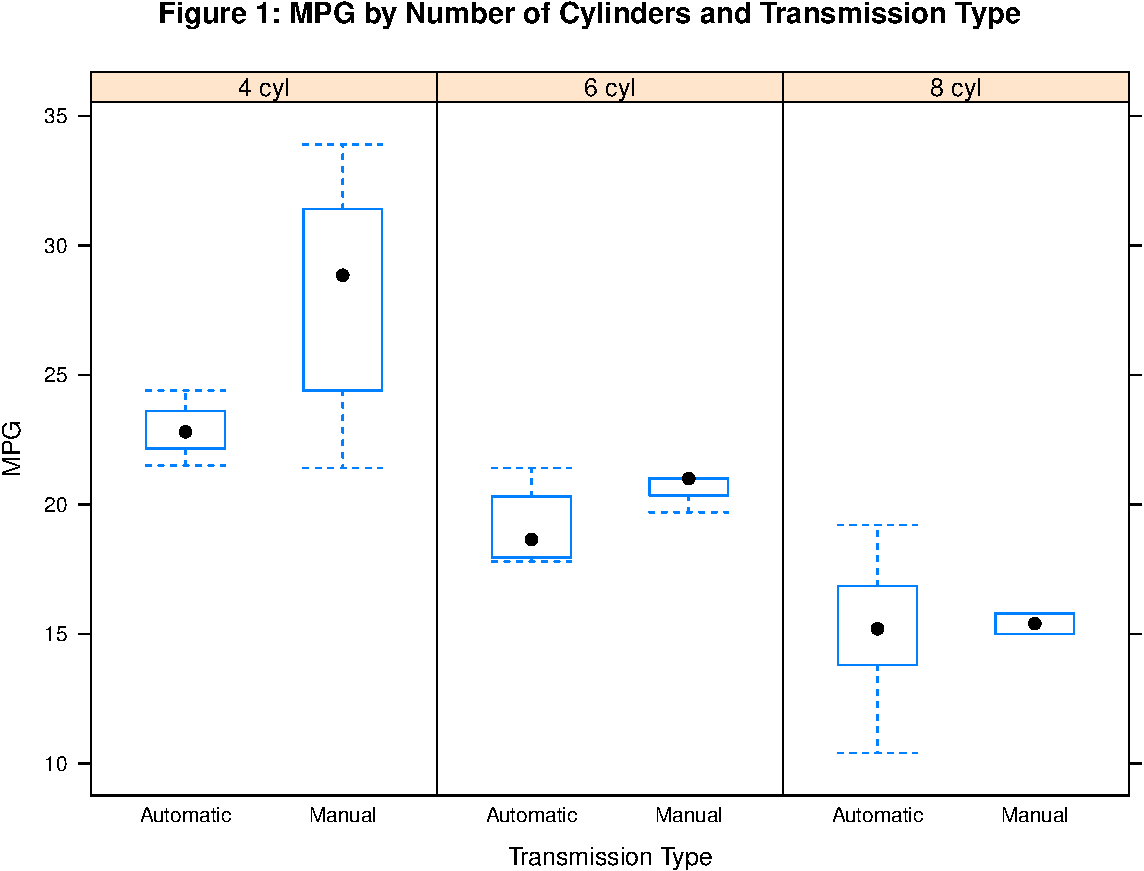
\includegraphics{mtcars_files/figure-latex/boxplot-1.pdf}

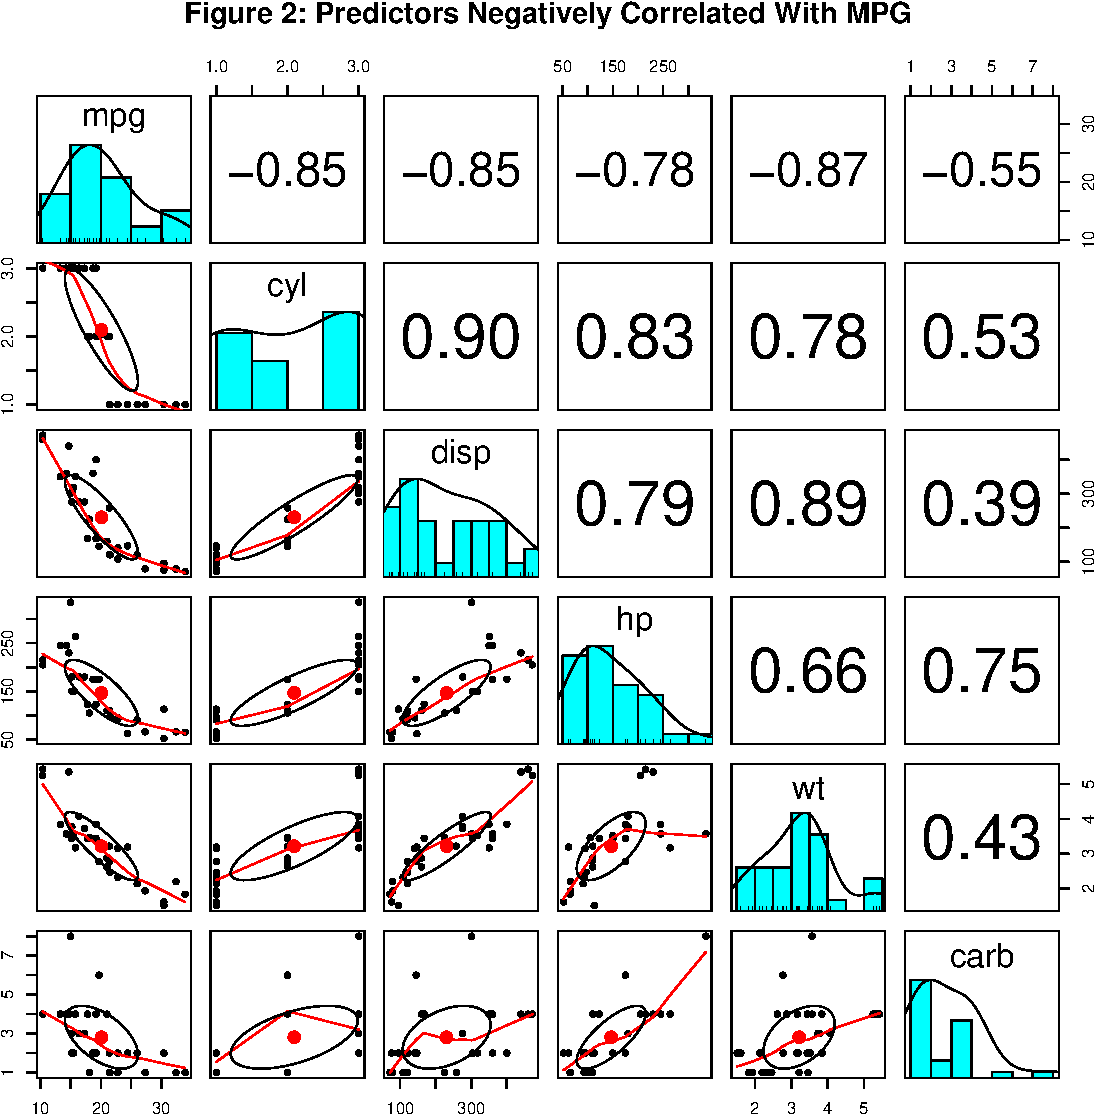
\includegraphics{mtcars_files/figure-latex/scatterplot1-1.pdf}

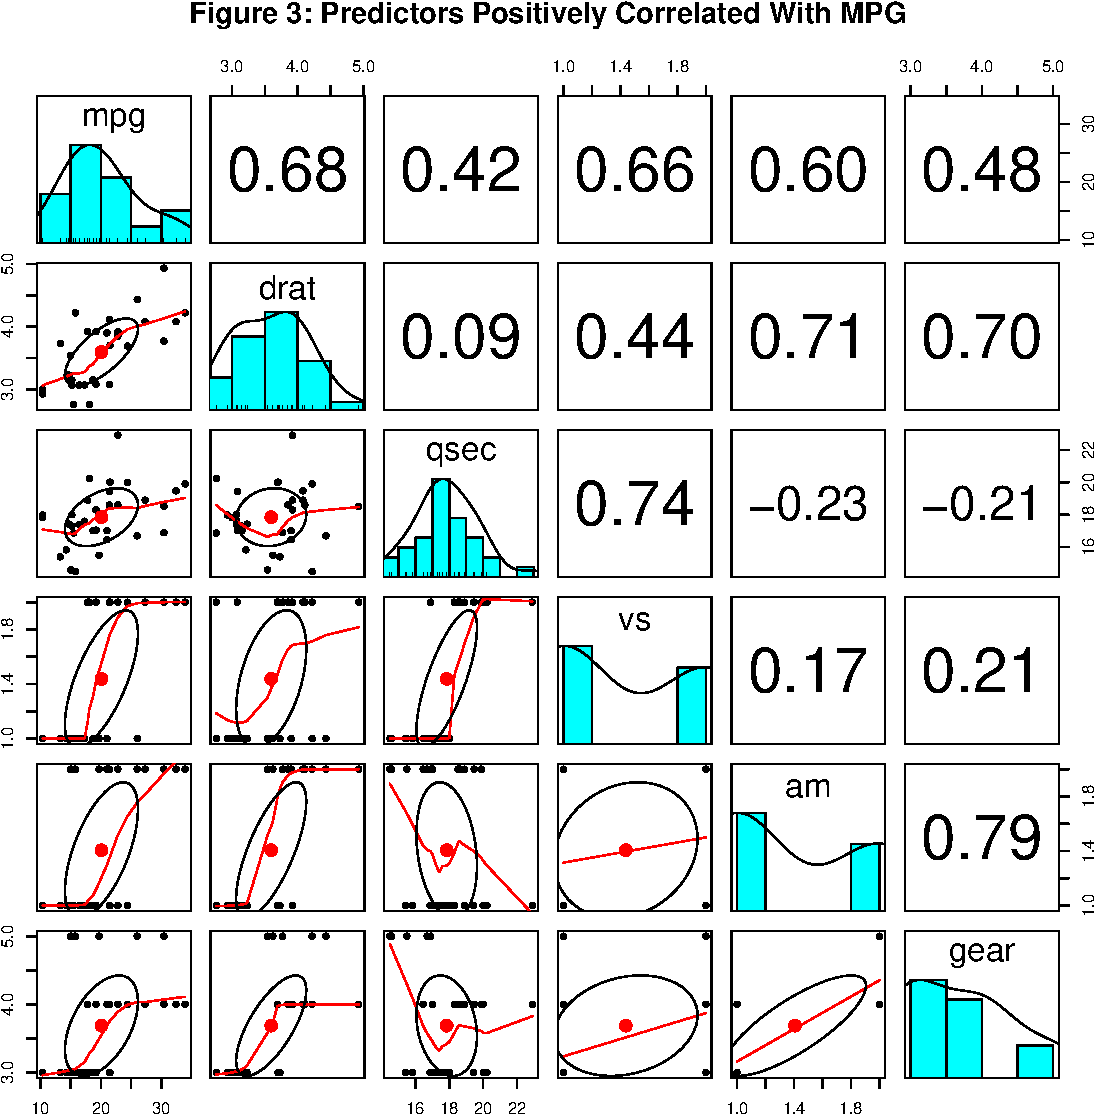
\includegraphics{mtcars_files/figure-latex/scatterplot2-1.pdf}

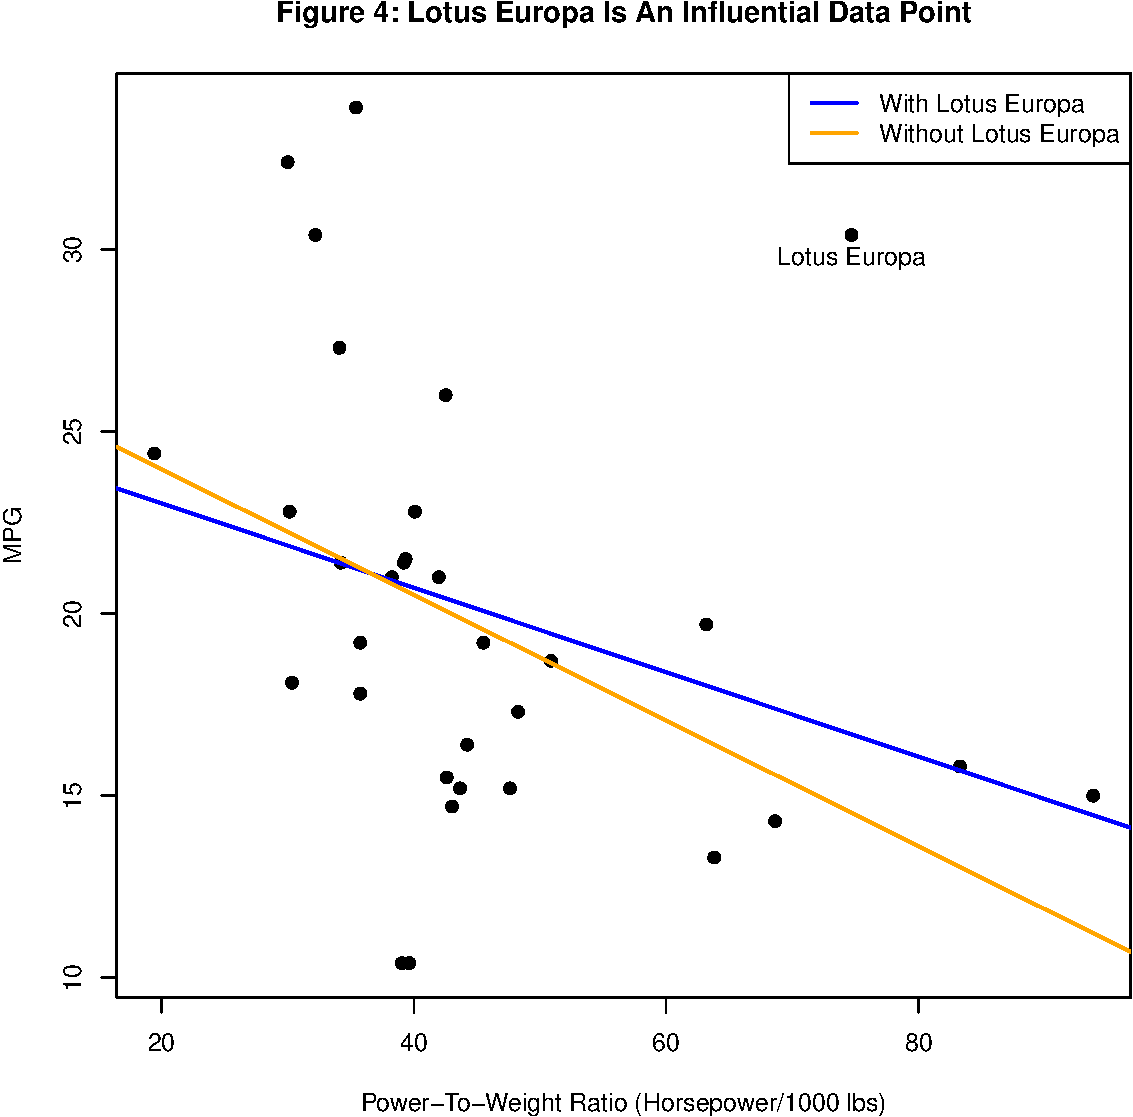
\includegraphics{mtcars_files/figure-latex/scatterplot3-1.pdf}

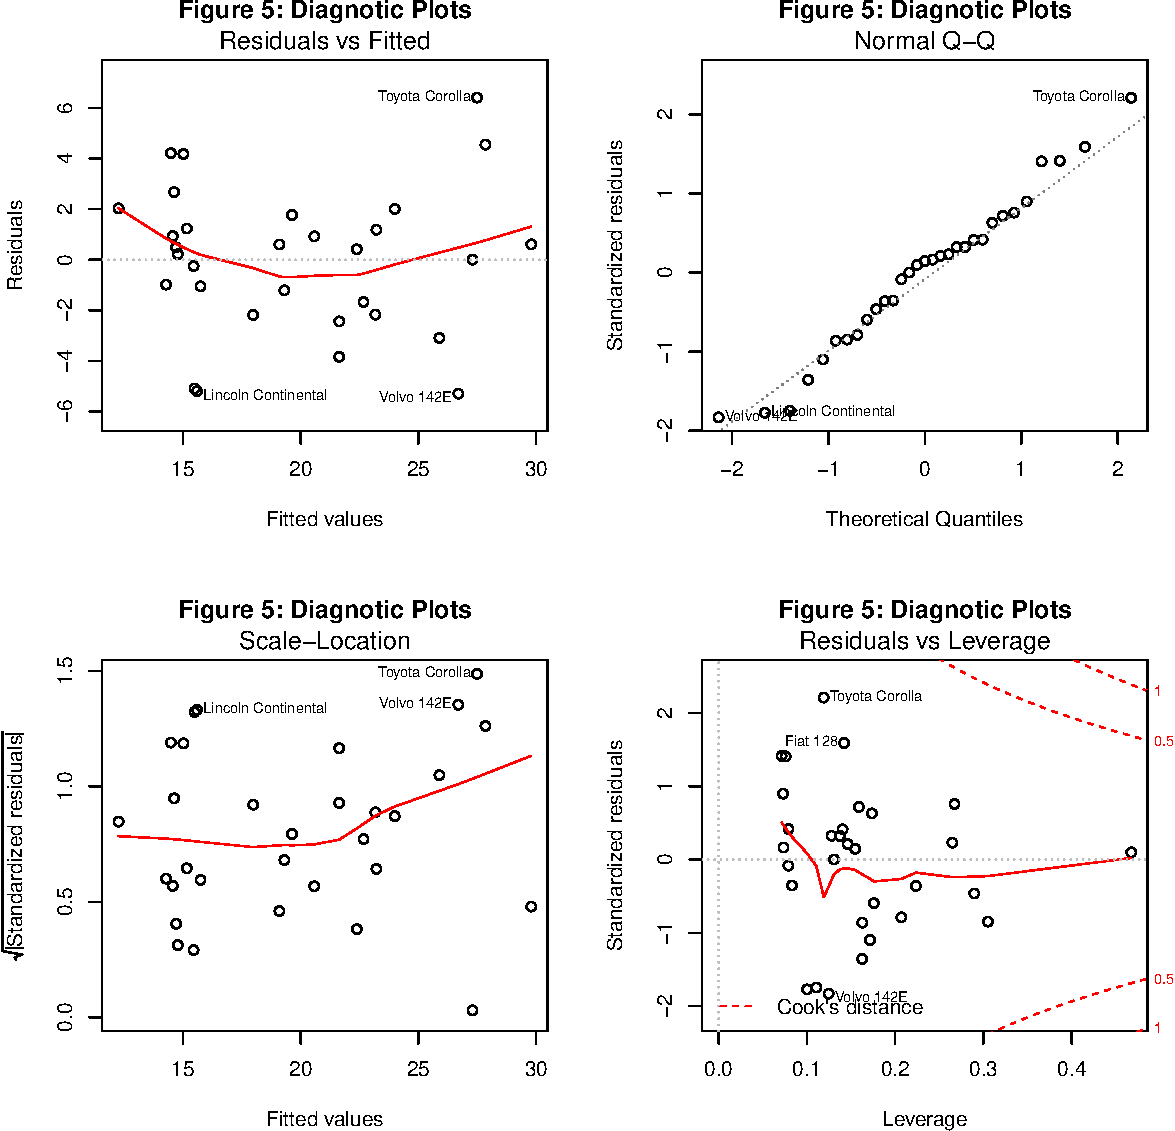
\includegraphics{mtcars_files/figure-latex/diagnostic-1.pdf}

\end{document}
